\documentclass[11pt]{article}
\usepackage[margin=1in]{geometry}
\usepackage{amsmath,amssymb,amsfonts,bm}
\usepackage{booktabs,multirow,array}
\usepackage{graphicx}
\graphicspath{{figures/screening_resolution/}}
\usepackage{xcolor}
\usepackage{hyperref}
\usepackage{cleveref}
\usepackage{siunitx}
\usepackage{enumitem}
\usepackage{microtype}
\usepackage{authblk}
\usepackage{placeins}
\emergencystretch=3em
\hypersetup{colorlinks=true,linkcolor=blue!60!black,citecolor=blue!60!black,urlcolor=blue!60!black}
\newcommand{\E}{\mathbf{e}}
\newcommand{\norm}[1]{\left\lVert #1 \right\rVert}

% Point estimates and interval summaries are bound to the released result layer.
\newcommand{\PZeroFOneNaucc}{0.105}
\newcommand{\PZeroFOnePersistFive}{--}
\newcommand{\PZeroFThreePersistFive}{39\%}
\newcommand{\PZeroFThreeNaucc}{0.110}
\newcommand{\PZeroFFourNaucc}{0.106}
\newcommand{\PTwoFOneNaucc}{0.060}
\newcommand{\PTwoFThreeNaucc}{0.043}
\newcommand{\PTwoFFourNaucc}{0.046}
\newcommand{\PZeroFOneEliteNaucc}{0.003}
\newcommand{\PZeroFOneIntermediateNaucc}{0.076}
\newcommand{\PZeroFOneBroadNaucc}{0.145}
\newcommand{\PZeroFThreeEliteNaucc}{-0.000}
\newcommand{\PZeroFThreeIntermediateNaucc}{0.061}
\newcommand{\PZeroFThreeBroadNaucc}{0.160}
\newcommand{\PZeroFFourEliteNaucc}{-0.004}
\newcommand{\PZeroFFourIntermediateNaucc}{0.069}
\newcommand{\PZeroFFourBroadNaucc}{0.151}
\newcommand{\PTwoFOneEliteNaucc}{-0.023}
\newcommand{\PTwoFOneIntermediateNaucc}{0.030}
\newcommand{\PTwoFOneBroadNaucc}{0.095}
\newcommand{\PTwoFThreeEliteNaucc}{-0.021}
\newcommand{\PTwoFThreeIntermediateNaucc}{-0.037}
\newcommand{\PTwoFThreeBroadNaucc}{0.089}
\newcommand{\PTwoFFourEliteNaucc}{-0.021}
\newcommand{\PTwoFFourIntermediateNaucc}{-0.024}
\newcommand{\PTwoFFourBroadNaucc}{0.089}
\newcommand{\PZeroFOneDualHighTenNaucc}{-0.046}
\newcommand{\PZeroFOneDualHighTenN}{58}
\newcommand{\PZeroVolumeDeltaTau}{0.722}
\newcommand{\PZeroVolumeDeltaNaucc}{0.813}
\newcommand{\PZeroBandGapDeltaTau}{0.663}
\newcommand{\PZeroBandGapDeltaNaucc}{0.792}
\newcommand{\PZeroFOneClusterNauccCI}{[0.056, 0.153]}
\newcommand{\PZeroFOneClusterQTenCI}{[-0.117, 0.165]}
\newcommand{\PZeroFOneClusterQFiftyCI}{[0.031, 0.325]}
\title{\textbf{CrossPiezo: Limited Elite-Set Reproducibility in Cross-Database Piezoelectric Screening}}
\author[1]{Anonymous Author(s)}
\affil[1]{Anonymous Institution}
\date{}
\begin{document}
\maketitle

\begin{abstract}
High-throughput materials screening assumes that top-ranked candidates are reproducible across databases, yet agreement is often reduced to a single global rank statistic.
We introduce CrossPiezo, a structure-matched benchmark of 573 materials shared by the Materials Project and JARVIS, and quantify screening resolution with three coordinate-invariant piezoelectric response scalars.
Across the P0 panel, the two sources share 0 of 5 materials in their top 1\%, 1 of 28 in their top 5\%, and 8 of 57 in their top 10\%; overlap increases only after substantially broadening the screened pool, and the qualitative pattern persists in the tighter 207-pair panel.
In contrast, unit-cell volume and band gap are markedly more reproducible across the same sources, consistent with substantially greater cross-workflow sensitivity of the piezoelectric response.
These results show that global rank association alone does not determine elite-set reproducibility in high-throughput piezoelectric screening.
\end{abstract}

\section{Introduction}
Piezoelectric response tensors are central to electromechanical materials design, yet costly to compute with density-functional perturbation theory (DFPT) \cite{baroni2001,choudhary2020ht}.
The Materials Project (MP) and JARVIS projects have released thousands of computed tensors \cite{dejong2015,choudhary2020}, and recent equivariant neural networks report strong in-source predictive agreement \cite{batzner2022,chen2022,choudhary2021,wen2024,dong2025}.
Improved agreement with a held-out subset of one database does not guarantee that a candidate is robustly ranked across independently generated high-throughput datasets \cite{choudhary2021uncertainty,choudhary2024leaderboard}.

We introduce \emph{screening resolution} as a diagnostic lens.
Rather than asking ``what is the average rank correlation between two sources?'' we ask ``at what elite fraction $q$ does the overlap between source-specific top-$q$ sets become reliably and meaningfully greater than its chance expectation?''
This distinction matters for materials discovery: a model validated only on aggregate correlation may still disagree with an independent source on the very candidates an experimenter would pursue \cite{yuan2018,ma2023,dong2025}.

This paper makes three contributions.
First, we release a frozen, structure-matched benchmark of 573 MP--JARVIS pairs and three coordinate-invariant response scalars.
Second, we show that cross-database concordance is resolution-dependent: near-chance in the elite tail, weak in the intermediate band, and only modest in the broad band.
Third, we demonstrate that scalar controls are far more consistent than the piezoelectric response, and retain source-robust portfolio constructions as an operational illustration of candidate coverage under two-source uncertainty.
The portfolio analysis is an operational illustration rather than a validated method comparison, an independent validation, or evidence of physical truth.

\section{CrossPiezo benchmark}
\label{sec:benchmark}

The CrossPiezo-Invariant-v1 panel contains P0 ($n=573$) and P2 ($n=207$) structure-matched pairs with identical or near-identical relaxed crystal structures across MP and JARVIS \cite{jain2013,ong2013}.
Figure~\ref{fig:benchmark_concept}a summarises the matching pipeline: 8,316 processed records were reduced to 1,266 structure-level overlaps, then to the frozen P0 and P2 panels.
Panel membership was fixed after a response-blind manual audit of the top-matched candidates using a frozen rule set; all audit decisions are recorded in the repository.

For each source we compute three coordinate-invariant scalars from the piezoelectric stress tensor $\E$ (Figure~\ref{fig:benchmark_concept}b):
F1 = Cartesian Frobenius norm $\norm{\E}_F$;
F3 = true collinear longitudinal maximum $\max_{\norm{\bm n}=1} |n_i e_{ijk} n_j n_k|$;
F4 = Kelvin/Mandel operator norm on symmetric strain.
F3 isolates the longitudinal single-crystal response; F1 and F4 quantify rotation-invariant tensor magnitude and maximum linear response, respectively, and are useful for norm-based screening.

Screening resolution is defined by sweeping the screened quantile $q$ from 1\% to 50\% and comparing the source-specific top-$q$ sets (Figure~\ref{fig:benchmark_concept}c).
At each $q$ we report the chance-adjusted Jaccard overlap $\widetilde J_q$ and a simultaneous 95\% confidence band; the area-averaged chance-adjusted Jaccard is denoted nAUCC for continuity (see Methods).
The key diagnostic is whether concordance is reliably sustained as the candidate pool narrows from broad (20--50\%) to elite (1--10\%).

\section{Elite-tail screening resolution}
\label{sec:resolution}

Figure~\ref{fig:screening_resolution_flagship} shows the flagship screening-resolution results.
On P0 the three functionals behave similarly: full-range nAUCC is \PZeroFOneNaucc{} for F1, \PZeroFThreeNaucc{} for F3 and \PZeroFFourNaucc{} for F4 (Table~\ref{tab:concordance}).
The unified reduced-formula cluster bootstrap gives a P0 F1 nAUCC of \PZeroFOneNaucc{} with 95\% CI \PZeroFOneClusterNauccCI{}; a five-quantile persistent practical-onset threshold at the prespecified $\delta=0.05$ level is not observed for F1.
The qualitative pattern persists in P2: F1 nAUCC = \PTwoFOneNaucc{}, F3 nAUCC = \PTwoFThreeNaucc{}, and F4 nAUCC = \PTwoFFourNaucc{}, although the smaller panel gives wider uncertainty.
Thus, even at the broad $q=50\%$ threshold, P0 F1 chance-adjusted Jaccard is only $0.178$ (simultaneous 95\% confidence-band interval \PZeroFOneClusterQFiftyCI{}); the lower band does not cross the prespecified practical threshold in a persistent run.

The banded partial nAUCC summary (Figure~\ref{fig:screening_resolution_flagship}, bottom row and Table~\ref{tab:concordance}) makes the resolution-dependence explicit.
On P0 F1, concordance is essentially absent in the elite band (partial nAUCC = \PZeroFOneEliteNaucc{}), modest in the intermediate band (\PZeroFOneIntermediateNaucc{}), and only clearly positive in the broad band (\PZeroFOneBroadNaucc{}).
The same graded pattern holds for F3 and F4 and is preserved, though attenuated, on P2.

Corrected high-response sensitivity analyses avoid the pooled-selection collider bias (Supplementary Table~S1).
The dual-high subset ($f=0.10$, $N=\PZeroFOneDualHighTenN{}$) has nAUCC = \PZeroFOneDualHighTenNaucc{}, and the JARVIS- and MP-anchor subsets give consistently weak or negative elite-tail concordance.
These sensitivity analyses support the conclusion that the elite-tail resolution gap is not an artifact of the high-response definition.

\begin{figure}[htbp]
\centering

\includegraphics[width=0.95\textwidth]{fig1_benchmark_concept}
\caption{CrossPiezo benchmark concept.
(a) Structure-matched data pipeline.
(b) The three coordinate-invariant piezoelectric response scalars computed from the stress tensor $\mathbf{e}$.
(c) Screening-resolution compares source-specific top-$q$ sets; concordance generally grows as the screened pool broadens.
(d) Main finding: cross-database concordance is near-chance in the elite tail and only becomes modest in the broad band.}
\label{fig:benchmark_concept}
\end{figure}

\begin{figure}[htbp]
\centering
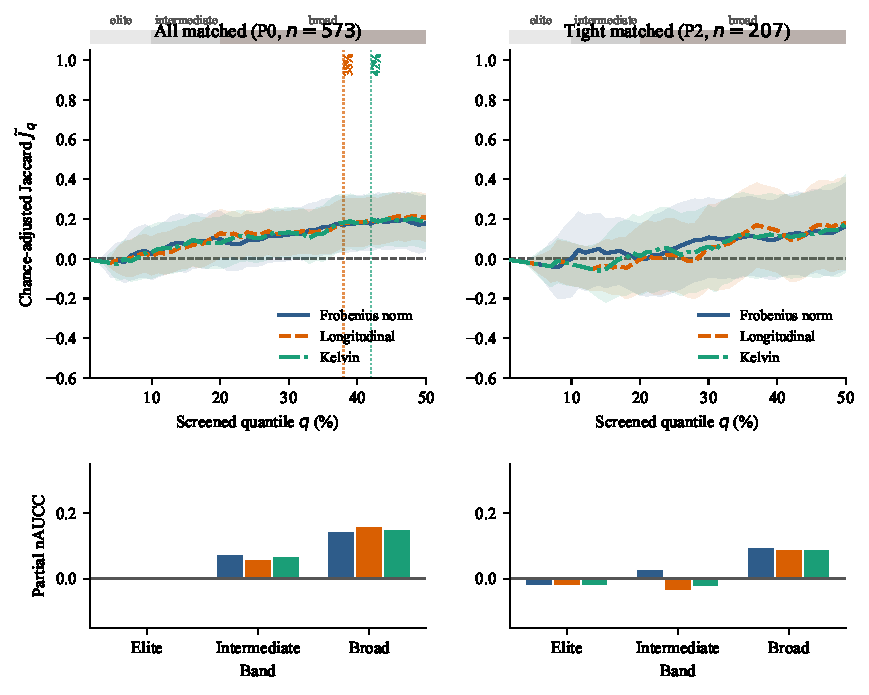
\includegraphics[width=0.95\textwidth]{fig2_screening_resolution_flagship}
\caption{Flagship screening-resolution results.
Top row: chance-adjusted Jaccard overlap $\widetilde J_q$ for P0 (left) and P2 (right), with simultaneous 95\% confidence bands.
Line styles distinguish the three invariants: Frobenius norm (solid), Longitudinal (dashed), Kelvin (dash-dot).
Light background regions indicate the elite, intermediate, and broad screening bands.
Bottom row: partial nAUCC by band; error bars are 95\% percentile intervals from the reduced-formula cluster bootstrap.}
\label{fig:screening_resolution_flagship}
\end{figure}

\begin{table}[htbp]
\centering
\caption{Screening-resolution summary. Full-range nAUCC and partial nAUCC by band for P0 ($n=573$) and P2 ($n=207$). $q_{0.05}^{\mathrm{persist}}$ requires five consecutive lower-confidence bounds above 0.05.}
\label{tab:concordance}
\begin{tabular}{llccccc}
\toprule
Panel & Metric & nAUCC & Elite & Intermediate & Broad & $q_{0.05}^{\mathrm{persist}}$ \\
\midrule
P0 & Frobenius norm & \PZeroFOneNaucc{} & \PZeroFOneEliteNaucc{} & \PZeroFOneIntermediateNaucc{} & \PZeroFOneBroadNaucc{} & \PZeroFOnePersistFive{} \\
P0 & Longitudinal & \PZeroFThreeNaucc{} & \PZeroFThreeEliteNaucc{} & \PZeroFThreeIntermediateNaucc{} & \PZeroFThreeBroadNaucc{} & \PZeroFThreePersistFive{} \\
P0 & Kelvin & \PZeroFFourNaucc{} & \PZeroFFourEliteNaucc{} & \PZeroFFourIntermediateNaucc{} & \PZeroFFourBroadNaucc{} & 42\% \\
\midrule
P2 & Frobenius norm & \PTwoFOneNaucc{} & \PTwoFOneEliteNaucc{} & \PTwoFOneIntermediateNaucc{} & \PTwoFOneBroadNaucc{} & -- \\
P2 & Longitudinal & \PTwoFThreeNaucc{} & \PTwoFThreeEliteNaucc{} & \PTwoFThreeIntermediateNaucc{} & \PTwoFThreeBroadNaucc{} & -- \\
P2 & Kelvin & \PTwoFFourNaucc{} & \PTwoFFourEliteNaucc{} & \PTwoFFourIntermediateNaucc{} & \PTwoFFourBroadNaucc{} & -- \\
\bottomrule
\end{tabular}
\end{table}

\FloatBarrier
\section{Response properties are unusually workflow-sensitive}
\label{sec:controls}

If the elite-tail gap were a generic failure of structure matching, all properties should show similarly weak cross-source concordance.
They do not.
Figure~\ref{fig:control_forest} compares piezoelectric F1 against unit-cell volume, band gap, energy above hull and dielectric trace.
Volume is the strongest control (P0 Kendall $\tau=0.967$, nAUCC $=0.918$), followed by band gap ($\tau=0.908$, nAUCC $=0.897$).
All controls have positive $\Delta\tau$ and higher nAUCC than F1; energy above hull is flagged for a high fraction of identical cross-source values, largely associated with tied zero-hull entries. This flag does not establish copying (open circle in Figure~\ref{fig:control_forest}).

This contrast is consistent with substantially greater cross-workflow sensitivity of the piezoelectric response.
It does not prove that response disagreement is mainly conventional; an irreducible physical component cannot be ruled out without an independent third protocol or experiment.

\begin{figure}[htbp]
\centering

\includegraphics[width=0.95\textwidth]{fig3_control_forest}
\caption{Property-control comparison on P0.
Left: advantage of each control over piezoelectric F1 in Kendall $\tau$, with 95\% confidence intervals.
Right: absolute nAUCC for each control, with the dashed line and shaded band showing the F1 nAUCC point estimate and 95\% CI.
All controls are substantially more cross-source consistent than the piezoelectric response.
The energy-above-hull control is marked with an open circle because many stable materials share a zero hull value in both sources.}
\label{fig:control_forest}
\end{figure}

\section{Discussion}
\label{sec:discussion}

The practical consequence of the resolution gap is that single-source elite lists are not automatically reproducible.
Supplementary Figures~S1--S2 and Tables~S3--S4 illustrate candidate-selection ambiguity and an operational source-robust portfolio analysis.
Because the portfolio objective is defined using the two observed source lists, its apparent coverage gain is target-aligned and does not establish out-of-sample robustness or physical correctness.

\subsection{Screening resolution versus global rank correlation}

The weak elite-tail resolution is a statement about the reproducible resolution of these two databases, not about the physical correctness of either source.
A model can achieve strong aggregate agreement on a held-out subset of one database while still disagreeing with an independent source on the specific candidates a human experimenter would pursue.
On P0 F1 the global Kendall $\tau$ is only $0.245$ and Spearman $\rho$ is $0.350$; more importantly, the top-$5\%$ precision is $0.036$ and the chance-adjusted Jaccard at $q=10\%$ is $0.024$ (simultaneous 95\% confidence-band interval \PZeroFOneClusterQTenCI{}), essentially indistinguishable from chance (Supplementary Tables~S5 and S7 and Figure~S4).
We recommend that future high-throughput screening reports screening-resolution curves, chance-adjusted overlaps, banded partial nAUCC and multi-source coverage diagnostics alongside aggregate correlations and global rank correlations.

\subsection{Why response properties are more workflow-sensitive}

Simpler scalar observables such as unit-cell volume and band gap are reproduced far more reliably across MP and JARVIS than the piezoelectric tensor.
This pattern is consistent with higher workflow sensitivity for response tensors: piezoelectric constants depend on density-functional settings, strain conventions, finite-difference or DFPT details, and post-processing choices that are not fully aligned between the two databases.
The control contrast does not establish that conventions dominate; an irreducible physical disagreement cannot be ruled out without a third independent protocol or experiment.

\subsection{Consequences for AI-guided materials selection}

For AI-guided discovery, our results imply that a model trained and validated on a single high-throughput source may inherit that source's idiosyncrasies.
Elite candidates selected from a single source should not automatically be treated as robustly high-performing.
The source-robust portfolio analysis is therefore retained only as an operational illustration: its worst-source coverage objective is aligned with the balanced-union construction, so it is not evidence of a validated method comparison or a guarantee of physical correctness.

\subsection{Limits of two-source evidence}

Our conclusions are source-pair specific.
Only MP and JARVIS are compared, and full workflow harmonisation was not possible.
Elite-tail samples are small (exactly 5 materials in P0 and 2 in P2 under the prespecified floor rule), so elite-tail statements are lower-bound diagnostics rather than precise population estimates.
A 48-material third-protocol adjudication plan is specified in the repository, but no independent third-protocol calculation is included in this study.
Experimental adjudication would be required to settle source correctness on specific candidates \cite{wilkinson2016,choudhary2024leaderboard}.

\section{Methods}
\label{sec:methods}

\paragraph{Paired universe.}
P0 and P2 were built by structure matching of relaxed CIFs followed by a response-blind manual audit of the top candidates using a frozen rule set; full details and the frozen membership file are released in the repository.
The frozen matcher tolerances are: fractional length tolerance $\ell_\mathrm{tol}=0.2$, site tolerance $s_\mathrm{tol}=0.3$\,\AA, angle tolerance $5^\circ$, primitive-cell reduction enabled, and lattice scaling enabled.
P0 ($n=573$) is the full set of accepted structure matches; P2 ($n=207$) is the subset passing tighter RMS-distance and lattice-distance thresholds ($\mathrm{RMS}_\mathrm{thr}\approx0.0078$\,\AA, lattice-distance threshold $\approx0.0036$).
A single auditor made all response-blind decisions; ambiguous cases were quarantined and recorded.
At the 1\% elite quantile the prespecified floor rule gives exactly 5 materials in P0 and 2 materials in P2.
The association between relaxed-structure distance and the observed rank discrepancy is statistically detectable at this panel size but negligible in magnitude (Spearman $\rho=-0.09$, $p=0.0312$; Supplementary Figure~S5); this is a sensitivity diagnostic rather than an exclusion of threshold or matching-error effects.

\paragraph{Response functionals.}
For each source we compute three coordinate-invariant scalars from the piezoelectric stress tensor $\E$ \cite{nye1957}.
Using the orthonormal Mandel representation
\[
M = \begin{bmatrix}
e_{1xx} & e_{1yy} & e_{1zz} & \sqrt{2}e_{1yz} & \sqrt{2}e_{1xz} & \sqrt{2}e_{1xy}\\
e_{2xx} & e_{2yy} & e_{2zz} & \sqrt{2}e_{2yz} & \sqrt{2}e_{2xz} & \sqrt{2}e_{2xy}\\
e_{3xx} & e_{3yy} & e_{3zz} & \sqrt{2}e_{3yz} & \sqrt{2}e_{3xz} & \sqrt{2}e_{3xy}
\end{bmatrix},
\]
and $m(\bm n)=(n_x^2,n_y^2,n_z^2,\sqrt{2}n_yn_z,\sqrt{2}n_xn_z,\sqrt{2}n_xn_y)^\mathsf{T}$ for $\|\bm n\|_2=1$, we define
\[
F_1=\|M\|_F,\qquad F_4=\|M\|_2=\sigma_{\max}(M),\qquad
F_3=\max_{\|\bm n\|_2=1}|\bm n^\mathsf{T}M m(\bm n)|.
\]
The internal check $0\leq F_3\leq F_4\leq F_1$ follows from these definitions; the convention audit verifies the corresponding tensor conversions and rotation invariances.

\paragraph{Source conventions and validation.}
Both databases report the piezoelectric stress tensor $\E$ in C/m$^2$ with the same Voigt order ($xx,yy,zz,yz,xz,xy$) and engineering-shear factor-of-two convention.
JARVIS values are expressed in the source-structure Cartesian frame; MP values are expressed in the MP IEEE-oriented structure frame.
Before comparison, MP structures are aligned to JARVIS structures using the frozen matcher and the recovered rotation is applied to the MP Cartesian tensor; F1, F3 and F4 are coordinate-frame invariants and are therefore unaffected by the source-specific frame choice.
Calculation settings not documented in the release metadata---exchange--correlation functional, pseudopotentials, DFPT vs finite-difference, cutoffs, k-points, relaxation thresholds, primitive/conventional defaults, and sign-convention history---are reported as unknown rather than assumed identical (see \path{docs/SCIENTIFIC_CONTRACT.md}).
A repository convention audit (\path{scripts/run_convention_audit.py}) confirms rotation invariance of F1/F3/F4, internal consistency of Voigt/Cartesian conversion and shear-factor handling, and convergence of the F3 optimiser to a dense-grid oracle; this rules out low-level convention errors in the CrossPiezo pipeline but does not prove that the two sources used identical calculation settings.

\paragraph{Chance-adjusted concordance curve.}
For equations below, $q$ is written as a fraction; the reported grid is $q=1\%,2\%,\dots,50\%$.
For a panel of size $N$, let $k(q)=\max\{1,\lfloor qN\rfloor\}$ and let $T_A(q)$ and $T_B(q)$ be the two top-$k(q)$ sets. With $X_q=|T_A(q)\cap T_B(q)|$,
\[
J_q=\frac{X_q}{2k(q)-X_q}.
\]
Under independent random rankings, $X_q\sim\operatorname{Hypergeom}(N,k,k)$ and the exact null expectation is
\[
E_0[J_q]=\sum_{x=\max(0,2k-N)}^k
\frac{x}{2k-x}\frac{\binom{k}{x}\binom{N-k}{k-x}}{\binom{N}{k}},
\]
not $J_q$ evaluated at $E[X_q]$. We report the chance-adjusted overlap
\begin{equation}
\widetilde J_q = \frac{J_q - E_0[J_q]}{1 - E_0[J_q]}.
\end{equation}
Thus $\widetilde J_q=0$ corresponds to the independent-ranking expectation and $\widetilde J_q=1$ to complete agreement; it may be negative, so the area summary below is not restricted to $[0,1]$.
We retain nAUCC as a compact name for the area-averaged adjusted Jaccard:
\begin{equation}
\mathrm{nAUCC} = \frac{1}{q_{\max}-q_{\min}} \int_{q_{\min}}^{q_{\max}} \widetilde J(q) \,dq.
\end{equation}
For a band $B=[q_\ell,q_u]$, the reported discrete estimate is
\[
\widehat A_B=\frac{1}{q_u-q_\ell}\sum_{j:[q_j,q_{j+1}]\subset B}
\frac{q_{j+1}-q_j}{2}\left(\widetilde J_{q_j}+\widetilde J_{q_{j+1}}\right).
\]
We distinguish two onset concepts. The persistent above-chance onset is $q^{\mathrm{persist}}_{0}=\min\{q_j:\operatorname{LCB}(q_{j+r})>0,\ r=0,\ldots,L-1\}$, whereas the prespecified persistent practical-onset threshold is $q^{\mathrm{persist}}_{0.05}=\min\{q_j:\operatorname{LCB}(q_{j+r})>0.05,\ r=0,\ldots,L-1\}$. We use $L=5$ and report $q^{\mathrm{persist}}_{0.05}$ as the primary practical threshold; $0.05$ is a prespecified practical threshold, not the unique criterion for statistical distinguishability from chance.
The primary curve and onset use a reduced-formula cluster bootstrap \cite{efron1994,romano2005}: groups are resampled with replacement, the bootstrap universe size and exact hypergeometric null are recomputed for every replicate, and the curve band uses a studentized sup-norm critical value. The original row-bootstrap curve is retained as a legacy sensitivity analysis; scalar nAUCC and partial nAUCC intervals use percentile intervals from the same primary replicates.

\paragraph{Banded reporting.}
The 1--50\% curve is split into elite (1--10\%), intermediate (10--20\%) and broad (20--50\%) bands. Partial nAUCC estimates and percentile-bootstrap intervals are reported for each band; simultaneous coverage applies to the confidence band for the full screening-resolution curve.

\paragraph{Conventional ranking diagnostics.}
For comparison with screening resolution we report standard top-$k$ and listwise diagnostics at $q=1\%,5\%,10\%,20\%,50\%$: plain Jaccard $J_q$, chance-adjusted Jaccard $\widetilde J_q$, precision@$k$ (equal here to recall@$k$ and the overlap coefficient), Rank-Biased Overlap with $p=0.95$, top-weighted Kendall $\tau$ on the union of the two top-$k$ sets, top-weighted Spearman $\rho$ on the same union, and the global Kendall $\tau$ and Spearman $\rho$ of the full paired rankings (Supplementary Table~S5 and Figure~S4).
These metrics illustrate that global rank association and elite-set agreement answer different questions; global rank association alone does not determine elite-tail reproducibility.

\paragraph{Corrected high-response sensitivity.}
High-response sensitivity uses three prespecified definitions:
(i) \texttt{dual\_high}: both source values exceed the $1-f$ quantile of $\min(F_J,F_M)$;
(ii) \texttt{jarvis\_anchor}: top $f$ by JARVIS, evaluated on MP;
(iii) \texttt{mp\_anchor}: top $f$ by MP, evaluated on JARVIS.
The legacy pooled selection is retained only as an exploratory check with a conditional permutation.

\paragraph{Controls and provenance.}
We compare piezoelectric response against volume, band gap, energy above hull and dielectric trace.
For each attribute we record source field, source database, unit, calculation type/version, missingness and a high identical-value fraction flag; this flag does not establish copying or shared provenance \cite{wilkinson2016}.
Absolute $\tau$ and nAUCC estimates are reported with grouped paired-bootstrap confidence intervals. The control differences $\Delta\tau = \tau_{\text{control}} - \tau_{\text{piezo}}$ and $\Delta\mathrm{nAUCC}$ are reported as full-panel point estimates in the comparison table; no confidence interval is claimed for these differences. Permutation $p$-values are retained in the result tables for audit, but no FDR-adjusted significance claim is made in the manuscript.

\paragraph{Robust portfolio benchmark.}
We fix an elite fraction $q^*=10\%$ and evaluate strategies on the full panel at budget factors $b=1.0$, 1.5 and 2.0.
Strategies include single-source, average percentile, maximin percentile, balanced union and a greedy minimax oracle \cite{dwork2001,clemen1986}; duplicate strategies with identical outputs are not repeated in the main interpretation.
The primary summary metric is worst-source recall (material-level). Results are reported only as an operational illustration in the Supplementary Information because the objective is defined from the two observed source lists.
Confidence intervals for paired differences versus the better single source are obtained from a full-procedure grouped bootstrap: reduced-formula groups are resampled with replacement, distinct bootstrap identities are assigned to duplicated occurrences, and portfolio selection, baseline selection and worst-source recall are recomputed within each replicate.
Earlier group-mean and conditional fixed-selection differences are retained in the repository for audit but are not used for the primary claim.
5-fold naive cross-evaluation by hashed pair identifier is also performed; CV estimates should be interpreted as an optimistic upper bound because different structural entries of the same reduced formula may leak across folds.

\section{Data availability}
\label{sec:data}
Hash-bound result tables, panel membership, the analysis manifest, convention-audit reports, the manuscript-numbers JSON and reproducibility instructions are released in the CrossPiezo repository.
A permanent archive containing the frozen manifest, all CSV artifacts, figures and the figure-generation script has been prepared for Zenodo/Figshare deposit; a private reviewer link will be provided before submission.

\begingroup
\small
\bibliographystyle{unsrt}
\bibliography{CrossPiezo_ScreeningResolution_references}
\endgroup
\end{document}
